\documentclass[aspectratio=169]{beamer}
\usetheme{Madrid}
\setbeamertemplate{navigation symbols}{}
\usecolortheme{default}
\usepackage{graphicx}
\usepackage{caption}
\usepackage{booktabs}
\usepackage{tikz}
\usetikzlibrary{shapes.geometric, arrows.meta, positioning, fit, backgrounds, calc}

% Ensure content doesn't overlap with bottom title bar
\setbeamersize{text margin left=0.3cm,text margin right=0.3cm}

\title{AI-based Damage Detection for Power Grid Equipment with SaaS-oriented Design}
\subtitle{Midterm Defense}
\author{Yujie Feng}
\institute{Supervisor: Jin Hou}
\date{}

% Customize footline with three adaptive columns: author/institute, title, page number
\setbeamertemplate{footline}
{
  \leavevmode%
  \hbox{%
  \begin{beamercolorbox}[wd=0.3\paperwidth,ht=2.25ex,dp=1ex,left]{author in head/foot}%
    \usebeamerfont{author in head/foot}\hspace*{2ex}\insertshortauthor\hspace*{0.5em}\insertshortinstitute
  \end{beamercolorbox}%
  \begin{beamercolorbox}[wd=0.5\paperwidth,ht=2.25ex,dp=1ex,center]{title in head/foot}%
    \usebeamerfont{title in head/foot}\insertshorttitle
  \end{beamercolorbox}%
  \begin{beamercolorbox}[wd=0.2\paperwidth,ht=2.25ex,dp=1ex,right]{date in head/foot}%
    \usebeamerfont{date in head/foot}\insertframenumber{} / \inserttotalframenumber\hspace*{2ex}
  \end{beamercolorbox}%
  }%
  \vskip0pt%
}

\begin{document}

%------------------------------------------------
\begin{frame}
  \titlepage
\end{frame}

%------------------------------------------------
\begin{frame}
\frametitle{Outline}
\vspace{-5pt}
\begin{columns}
\column{0.48\linewidth}
\begin{enumerate}
  \item Project Overview
  \item Progress Summary
  \item Module A: Bird Nest Detection (Completed)
  \item Module B: Oil Leak Detection (Trained \& Deployed)
\end{enumerate}

\column{0.48\linewidth}
\begin{enumerate}
  \setcounter{enumi}{4}
  \item Module C: Infrared High-Temperature Detection (Integrated)
  \item SaaS Flask Microservice Platform
  \item Problems \& Challenges
  \item Next Phase Work Plan
\end{enumerate}
\end{columns}
\end{frame}

%------------------------------------------------
\begin{frame}
\frametitle{Project Overview: A Scalable SaaS Inspection Platform}
\vspace{-5pt}
\small
\begin{columns}
\column{0.32\linewidth}
\textbf{Multi-modal Inputs}
\begin{itemize}
  \item UAV RGB imagery
  \item Infrared imagery
  \item Sensor telemetry streams
  \item Historical inspection records
\end{itemize}

\column{0.36\linewidth}
\textbf{AI Platform Core}
\begin{itemize}
  \item SaaS backend
    \begin{itemize}
      \item unified auth / RBAC
      \item multi-tenant isolation
      \item task queue / data lake
    \end{itemize}
  \item AI model registry
    \begin{itemize}
      \item Module A: Bird Nest Detection {\color{green!70!black}(Done)}
      \item Module B: Oil Leak Detection {\color{orange!80!black}(In progress)}
      \item Module C: Infrared High-Temp. {\color{orange!80!black}(Integrated)}
    \end{itemize}
\end{itemize}

\column{0.32\linewidth}
\textbf{Enterprise Outputs}
\begin{itemize}
  \item Alert Center (Dashboards)
  \item Work Order Dispatch
  \item Visual Analytics Portal
  \item API Integration
\end{itemize}
\end{columns}
\end{frame}

%------------------------------------------------
\begin{frame}
\frametitle{Midterm Progress Summary}
\vspace{-5pt}
\small
\begin{block}{Strategy: ``Vertical Slice First, then Horizontal Scale''}
Complete one module end-to-end before extending to multi-module registry and unified scheduling.
\end{block}
\vspace{4pt}
\begin{columns}[T]
\column{0.32\linewidth}
\textbf{\color{green!70!black}Module A (Completed)}
\begin{itemize}
  \item Mask R-CNN (Segm.)
  \item Bbox AP$_{50}$ = 1.0
  \item Flask Deployed
  \item \textbf{Status:} End-to-end PoC
\end{itemize}

\column{0.32\linewidth}
\textbf{\color{orange!80!black}Module B (In Progress)}
\begin{itemize}
  \item YOLOv8s (Det.)
  \item Trained: CSDN Data
  \item Best mAP50 $\approx$ 0.39
  \item \textbf{Status:} API Integrated
\end{itemize}

\column{0.32\linewidth}
\textbf{\color{orange!80!black}Module C (Integrated)}
\begin{itemize}
  \item OCR + Pixel Mapping
  \item Training-Free
  \item Custom Alarm Temp.
  \item \textbf{Status:} Visualized \& Deployed
\end{itemize}
\end{columns}
\end{frame}

%------------------------------------------------
\begin{frame}
\frametitle{Module A: Bird Nest Detection --- Data \& Model}
\vspace{-5pt}
\begin{columns}[T]
\column{0.48\linewidth}
\textbf{Dataset \& Augmentation}
\begin{itemize}
  \item \textbf{54 COCO Images:} Bbox + Polygons
  \item \textbf{Deterministic Augmentation:}
    \begin{itemize}
      \item Random IoU Crop (0.3--1.0)
      \item Photometric jitter 
      \item ResizeMax + PadSquare ($512\times512$)
    \end{itemize}
  \item $\rightarrow$ \textit{Avoids generative artifacts.}
\end{itemize}

\column{0.48\linewidth}
\textbf{Model \& Config}
\begin{itemize}
  \item \textbf{Arch:} Mask R-CNN (ResNet50 + FPNv2)
  \item \textbf{Opt:} AdamW ($5\times10^{-4}$) + OneCycleLR
  \item \textbf{Tech:} AMP Mixed Precision
  \item \textbf{Perf:} $\sim$27s/epoch, 70--85\% GPU
\end{itemize}
\end{columns}
\end{frame}

%------------------------------------------------
\begin{frame}
\frametitle{Module A: Bird Nest Detection --- Validation Metrics}
\vspace{-5pt}
\begin{columns}
\column{0.45\linewidth}
\textbf{COCO Validation Metrics}
\small
\begin{center}
\begin{tabular}{lcc}
\toprule
Metric & \textbf{bbox} & \textbf{segm} \\
\midrule
AP@[0.50:0.95] & 0.805 & 0.795 \\
AP50 & \textbf{1.000} & \textbf{1.000} \\
AP75 & 1.000 & 0.919 \\
AR@[0.50:0.95] & 0.837 & 0.828 \\
\bottomrule
\end{tabular}
\end{center}
\vspace{4pt}
\small Score threshold 0.4--0.5 gives optimal F1 trade-off in deployment.

\column{0.52\linewidth}
\centering
\includegraphics[width=0.90\textwidth,height=0.55\textheight,keepaspectratio]{../../assets/BirdNestDetectionResult.png}
\vspace{-4pt}
\captionof{figure}{Bird nest detection: bounding box and instance mask overlay.}
\end{columns}
\end{frame}

%------------------------------------------------
\begin{frame}
\frametitle{Module A: Bird Nest Detection --- Training Dynamics}
\vspace{-5pt}
\begin{columns}
\column{0.48\linewidth}
\centering
\includegraphics[width=0.95\textwidth]{../../../experiments/visualizations/loss_curves.png}
\vspace{-5pt}
\captionof{figure}{Train/Validation Loss Curves}

\column{0.48\linewidth}
\textbf{Key Observations}
\begin{itemize}
  \item Train: $1.41 \to 0.14$ $\mid$ Val: $0.65 \to 0.19$
  \item Plateaus $\sim$epoch 20 --- No Overfitting
  \item Right-skewed IoU: Strong Localization
  \item AR/AP drops gracefully at IoU 0.90
\end{itemize}
\end{columns}
\end{frame}

%------------------------------------------------
\begin{frame}
\frametitle{Module A: Bird Nest Detection --- PR \& Threshold Analysis}
\vspace{-5pt}
\begin{columns}
\column{0.48\linewidth}
\centering
\includegraphics[width=0.90\textwidth]{../../../experiments/visualizations/pr_curve_bbox_ap50.png}
\vspace{-5pt}
\captionof{figure}{Bbox PR Curves (IoU=0.50/0.75/0.90)}

\column{0.48\linewidth}
\centering
\includegraphics[width=0.90\textwidth]{../../../experiments/visualizations/threshold_sweep_bbox.png}
\vspace{-5pt}
\captionof{figure}{Score Threshold vs.\ P/R/F1 (IoU$\geq$0.5)}
\end{columns}
\vspace{2pt}
\small
\textit{With AP$_{50}$=1.0, threshold 0.4--0.5 optimizes F1; higher thresholds (0.6--0.8) trade recall for precision in deployment.}
\end{frame}

%------------------------------------------------
\begin{frame}
\frametitle{Module B: Oil Leak Detection --- Data \& Training Config}
\vspace{-5pt}
\begin{columns}[T]
\column{0.48\linewidth}
\textbf{Data Sources}
\begin{itemize}
  \item VOC ($\sim$103) + CSDN ($\sim$230)
  \item \texttt{prepare\_dataset.py} $\to$ Unified YOLO format
  \item Single class: \texttt{oil\_leak}
  \item \textbf{Current Run (train10):} CSDN Only
\end{itemize}

\column{0.48\linewidth}
\textbf{Training Config (YOLOv8s)}
\begin{itemize}
  \item \textbf{Arch:} \texttt{yolov8s.pt} (Single Class)
  \item \textbf{Hyper:} 150 epochs, batch 8, $640\times640$
  \item \textbf{Opt:} AdamW + Cosine LR
  \item \textbf{Aug:} Mosaic (0.3), Mixup (0.05)
\end{itemize}
\end{columns}
\end{frame}

%------------------------------------------------
\begin{frame}
\frametitle{Module B: Oil Leak Detection --- Validation Metrics}
\vspace{-5pt}
\begin{columns}
\column{0.48\linewidth}
\textbf{Best Validation Results} (train10-csdn, epoch 93--94)
\small
\begin{center}
\begin{tabular}{lc}
\toprule
Metric & Value \\
\midrule
Precision(B) & $\approx$ 0.83 \\
Recall(B) & $\approx$ 0.34 \\
mAP50(B) & $\approx$ \textbf{0.39} \\
mAP50-95(B) & $\approx$ \textbf{0.26} \\
Total epochs run & 123 \\
\bottomrule
\end{tabular}
\end{center}
\vspace{4pt}
\small $\rightarrow$ High precision / low recall indicates conservative detection. Next step: Train on full merged data.

\column{0.48\linewidth}
\centering
\includegraphics[width=0.90\textwidth,height=0.55\textheight,keepaspectratio]{../../assets/OilLeakDetectionResult.png}
\vspace{-4pt}
\captionof{figure}{Oil leak detection: identified leakage region on equipment.}
\end{columns}
\end{frame}

%------------------------------------------------
\begin{frame}
\frametitle{Module B: Oil Leak Detection --- Training Results}
\vspace{-5pt}
\begin{columns}
\column{0.48\linewidth}
\centering
\includegraphics[width=0.95\textwidth]{../../../src/oil_leak/runs/detect/train10-csdn/results.png}
\vspace{-5pt}
\captionof{figure}{Training Results (loss / mAP curves)}

\column{0.48\linewidth}
\centering
\includegraphics[width=0.90\textwidth]{../../../src/oil_leak/runs/detect/train10-csdn/BoxPR_curve.png}
\vspace{-5pt}
\captionof{figure}{Validation PR Curve (IoU 0.5)}
\end{columns}
\end{frame}

%------------------------------------------------
\begin{frame}
\frametitle{Module B: Oil Leak Detection --- F1 \& Confusion Matrix}
\vspace{-5pt}
\begin{columns}
\column{0.48\linewidth}
\centering
\includegraphics[width=0.90\textwidth]{../../../src/oil_leak/runs/detect/train10-csdn/BoxF1_curve.png}
\vspace{-5pt}
\captionof{figure}{Validation F1 Curve}

\column{0.48\linewidth}
\centering
\includegraphics[width=0.90\textwidth]{../../../src/oil_leak/runs/detect/train10-csdn/confusion_matrix_normalized.png}
\vspace{-5pt}
\captionof{figure}{Normalized Confusion Matrix}
\end{columns}
\vspace{2pt}
\small
\textit{$\rightarrow$ Box-level detection identifies location; pixel-segmentation can be added if area tracking is needed.}
\end{frame}

%------------------------------------------------
\begin{frame}
\frametitle{Module C: Infrared High-Temperature Detection}
\vspace{-5pt}
\begin{columns}[T]
\column{0.48\linewidth}
\textbf{Approach: OCR Hybrid}
\begin{itemize}
  \item Deep-Learning Free
  \item EasyOCR: Parses temp scale
  \item Pixel-to-Temp Mapping
  \item \textbf{User Parameter:} Custom Alarm ($50^\circ$C)
\end{itemize}

\column{0.48\linewidth}
\textbf{Noise Suppression}
\begin{itemize}
  \item \textbf{Watermark Mask:} Ignores white logos
  \item \textbf{Legend Mask:} Excludes OCR regions
  \item \textbf{Result:} Outputs bounded hotspots + $\Delta$T
\end{itemize}
\end{columns}
\end{frame}

%------------------------------------------------
\begin{frame}
\frametitle{Module C: Infrared Detection --- Result}
\vspace{-5pt}
\begin{columns}
\column{0.48\linewidth}
\centering
\includegraphics[width=0.95\textwidth,height=0.70\textheight,keepaspectratio]{../../assets/InfraredHighTempDetection.png}
\vspace{-4pt}
\captionof{figure}{Hotspot bounding above user-defined threshold.}

\column{0.48\linewidth}
\centering
\includegraphics[width=0.95\textwidth,height=0.70\textheight,keepaspectratio]{../../assets/InfraredCard.png}
\vspace{-4pt}
\captionof{figure}{Infrared detection result card.}
\end{columns}
\end{frame}

%------------------------------------------------
\begin{frame}
\frametitle{SaaS Flask Microservice --- Platform Overview}
\vspace{-5pt}
\textbf{Architecture \& Request Flow}
\vspace{5pt}
\begin{center}
\resizebox{0.9\textwidth}{!}{
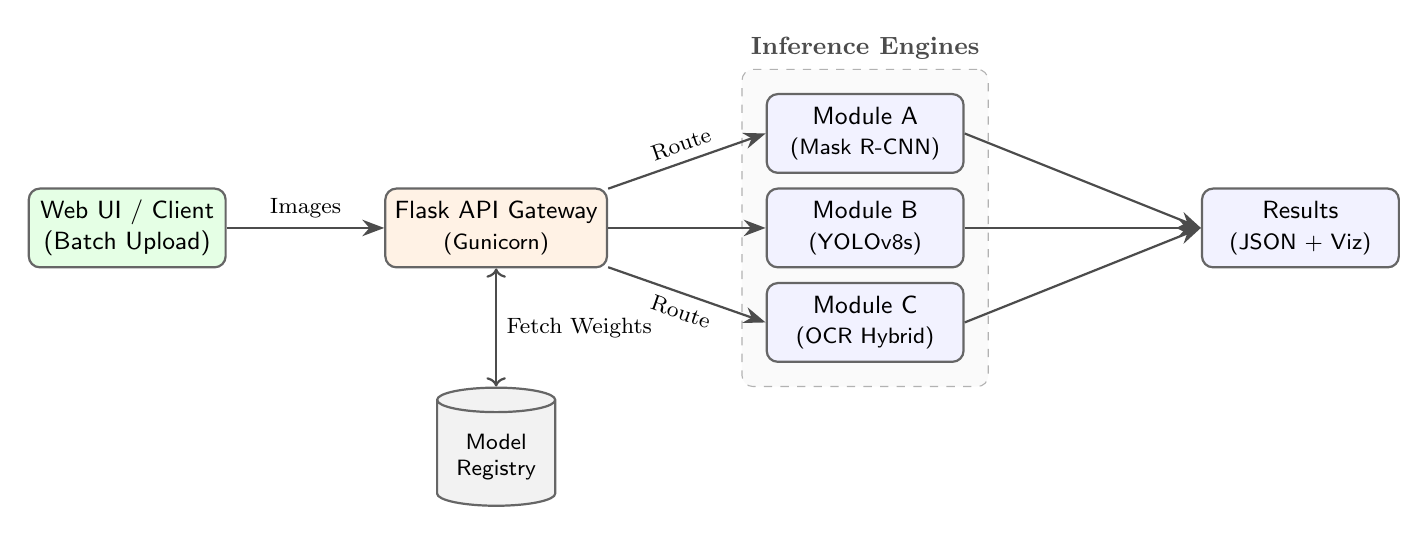
\begin{tikzpicture}[
  node distance=1.5cm and 2cm,
  box/.style={rectangle, draw=black!60, fill=blue!5, thick, rounded corners, minimum width=2.5cm, minimum height=1cm, align=center, font=\small\sffamily},
  db/.style={cylinder, draw=black!60, fill=gray!10, thick, aspect=0.25, minimum width=1.5cm, minimum height=1.5cm, align=center, shape border rotate=90, font=\footnotesize\sffamily},
  arrow/.style={-{Stealth[scale=1.2]}, thick, draw=black!70}
]

% Nodes
\node[box, fill=green!10] (client) {Web UI / Client \\ (Batch Upload)};
\node[box, right=of client, fill=orange!10] (api) {Flask API Gateway \\ \footnotesize(Gunicorn)};
\node[box, right=of api, yshift=1.2cm] (modelA) {Module A \\ \footnotesize(Mask R-CNN)};
\node[box, right=of api] (modelB) {Module B \\ \footnotesize(YOLOv8s)};
\node[box, right=of api, yshift=-1.2cm] (modelC) {Module C \\ \footnotesize(OCR Hybrid)};
\node[db, below=of api] (registry) {Model \\ Registry};
\node[box, right=of modelB, xshift=1cm] (output) {Results \\ \footnotesize(JSON + Viz)};

% Background Box for Inference Engine
\begin{scope}[on background layer]
  \node[draw=black!30, fill=black!2, dashed, rounded corners, fit=(modelA) (modelB) (modelC), inner sep=0.3cm, label={[font=\small\bfseries, text=black!70]above:Inference Engines}] (engines) {};
\end{scope}

% Arrows
\draw[arrow] (client) -- node[above, font=\footnotesize] {Images} (api);
\draw[arrow] (api) -- node[above, sloped, font=\footnotesize] {Route} (modelA.west);
\draw[arrow] (api) -- (modelB.west);
\draw[arrow] (api) -- node[below, sloped, font=\footnotesize] {Route} (modelC.west);
\draw[arrow, <->] (api) -- node[right, font=\footnotesize] {Fetch Weights} (registry);

\draw[arrow] (modelA.east) -- (output.west);
\draw[arrow] (modelB.east) -- (output.west);
\draw[arrow] (modelC.east) -- (output.west);

\end{tikzpicture}
}
\end{center}
\end{frame}

%------------------------------------------------
\begin{frame}
\frametitle{SaaS Platform --- User Interface}
\vspace{-5pt}
\begin{columns}
\column{0.48\linewidth}
\centering
\includegraphics[width=0.95\textwidth,height=0.35\textheight,keepaspectratio]{../../assets/LoginPage.png}
\vspace{-3pt}
\captionof{figure}{Login Interface}

\column{0.48\linewidth}
\centering
\includegraphics[width=0.95\textwidth,height=0.35\textheight,keepaspectratio]{../../assets/MainPage.png}
\vspace{-3pt}
\captionof{figure}{Main Dashboard \& Task Flow}
\end{columns}
\vspace{8pt}
\centering
\includegraphics[width=0.55\textwidth,height=0.28\textheight,keepaspectratio]{../../assets/HistroyPage.png}
\vspace{-3pt}
\captionof{figure}{History \& Statistical Analytics for Inference Records and Work Orders}
\end{frame}

%------------------------------------------------
\begin{frame}
\frametitle{Problems \& Challenges}
\vspace{-5pt}
\begin{block}{1. Generalization}
\begin{itemize}
  \item \textbf{Issue:} AP$_{50}$=1.0 on val set $\to$ Risk of performance drop in field (haze, new towers).
  \item \textbf{Action:} Integrate cross-scene data \& hard-sample mining across the platform.
\end{itemize}
\end{block}
\begin{block}{2. Technical Choices}
\begin{itemize}
  \item \textbf{SaaS:} Prioritize multi-model prototype over enterprise auth (OAuth2) for now.
  \item \textbf{Oil Leak:} YOLO box-level suffices; pixel-segmentation only if area stats needed.
\end{itemize}
\end{block}
\begin{block}{3. Constraints}
\begin{itemize}
  \item \textbf{Data:} Modest datasets ($\sim$50 bird nests, $\sim$300 oil leaks); annotation is bottleneck.
  \item \textbf{Deploy:} Flask multi-process works; true scale requires queue+worker pool.
\end{itemize}
\end{block}
\end{frame}

%------------------------------------------------
\begin{frame}
\frametitle{Next Phase Work Plan}
\vspace{-5pt}
\begin{columns}[T]
\column{0.48\linewidth}
\textbf{Track 1: SaaS Backend (Weeks 5--10)}
\begin{itemize}
  \item Multi-tenant RBAC \& Task Queue
  \item AI Model Registry API
  \item Productize training utilities
\end{itemize}

\column{0.48\linewidth}
\textbf{Track 2: Modules (Weeks 11--18)}
\begin{itemize}
  \item Oil Leak: Train on merged dataset
  \item Infrared: Multi-device adaptation
  \item Reuse data/training pipelines
\end{itemize}
\end{columns}
\vspace{8pt}
\begin{block}{Integration \& Defence (Weeks 19--20)}
\begin{itemize}
  \item End-to-end multi-user testing
  \item \textbf{Final Deliverable:} 3-Module SaaS Prototype + Thesis Report
\end{itemize}
\end{block}
\end{frame}

%------------------------------------------------
\begin{frame}
\frametitle{Discussion Points}
\vspace{-5pt}
\begin{enumerate}
  \item \textbf{Generalization strategy}: Should the project invest in cross-scene data collection or focus on augmentation and hard-sample mining to improve robustness of all three modules?
  \item \textbf{Oil leak improvement}: Current mAP50 $\approx$ 0.39 on CSDN dataset only. Should training be re-run on the merged VOC+CSDN dataset, or should the model architecture be upgraded (e.g.\ YOLOv8m / segmentation head)?
  \item \textbf{SaaS depth vs.\ breadth}: Should the final phase prioritize a fully functional RBAC and task-queue backend, or focus on expanding the AI modules and demo quality for the defence?
\end{enumerate}
\end{frame}

\end{document}
